%!TEX TS-program = lualatex
\documentclass[
	ngerman,
	twoside,
	pdfa=false,
	ruledheaders=section,%Ebene bis zu der die Überschriften mit Linien abgetrennt werden, vgl. DEMO-TUDaPub
	class=report,% Basisdokumentenklasse. Wählt die Korrespondierende KOMA-Script Klasse
	thesis={type=Übung},% Dokumententyp Thesis, für Dissertationen siehe die Demo-Datei DEMO-TUDaPhd
	accentcolor=TUDa-9d,% Auswahl der Akzentfarbe
	custommargins=false,% Ränder werden mithilfe von typearea automatisch berechnet
	marginpar=false,% Kopfzeile und Fußzeile erstrecken sich nicht über die Randnotizspalte
	%BCOR=5mm,%Bindekorrektur, falls notwendig
	parskip=half-,%Absatzkennzeichnung durch Abstand vgl. KOMA-Sript
	fontsize=11pt,%Basisschriftgröße laut Corporate Design ist mit 9pt häufig zu klein
%	logofile=tuda_logo.pdf, %Falls die Logo Dateien nicht installiert sind
]{tudapub}

% Sprachanpassung
\usepackage[english, main=ngerman]{babel}
\usepackage[autostyle]{csquotes}
\usepackage{microtype}
\usepackage{listings}
\usepackage{array}

% Literaturverzeichnis
\usepackage{biblatex}
\addbibresource{literature.bib}

% Pakete-Mathematik & mehr
\usepackage{mathtools}
\usepackage{amsmath}
\usepackage{amsfonts}
\usepackage{subcaption}
\usepackage{color}

% neu cmds
\newcommand*\diff{\mathop{}\!\mathrm{d}}
\newcommand*\Diff[1]{\mathop{}\!\mathrm{d^#1}}


\begin{document}
	\title{Software Engineering Übung 06}
	\subtitle{Design Prinzipien 2}
	\author[J. Lippert \and M. Dierking]
	{Jonathan Lippert \and Magnus Dierking}
	%\reviewer{}
	%\department{ce}

	
	\submissiondate{\today}
	

	\maketitle
	\pagenumbering{gobble}


	% Kurzzusammenfassung
%	\include{chapters/zusammenfassung}

	% Inhaltsverzeichnis 
%	\tableofcontents
	\newpage
	\pagenumbering{arabic}
	\setcounter{page}{1}
	

%-------------------------------------------------------------------------------------------------
     \chapter{Aufgabe}
\section*{a}
\subsection*{i}
Siehe Abbildung \ref{fig:graphLCOM}

\begin{figure}[h!]
	\centering
	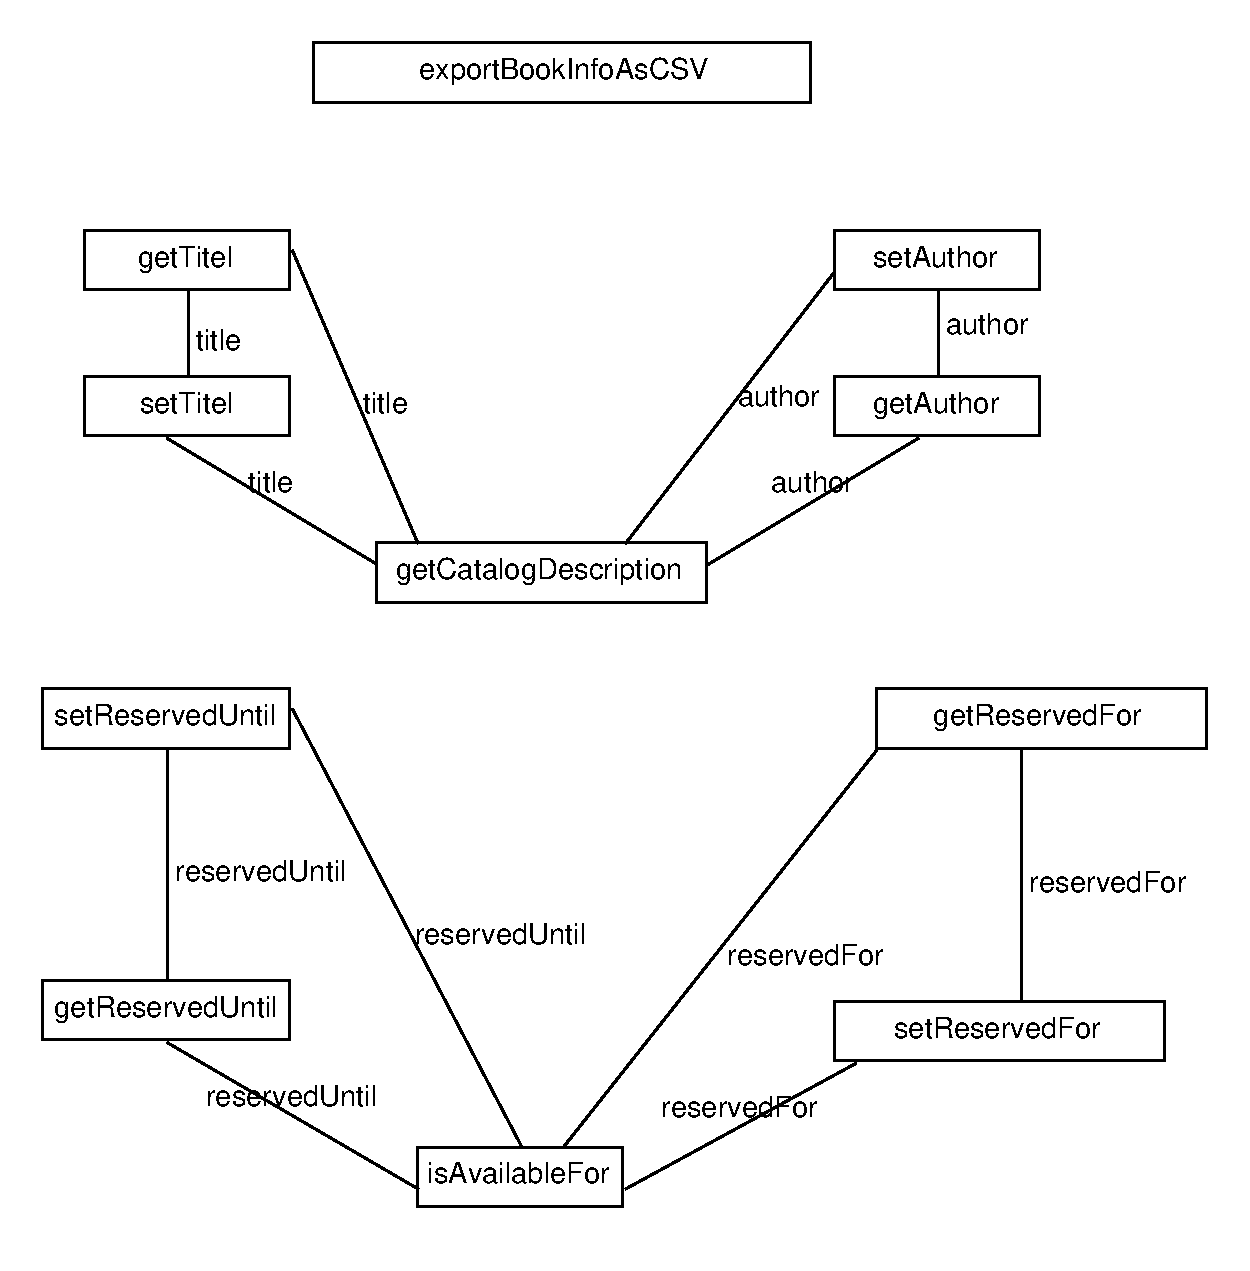
\includegraphics[width=0.8\textwidth, clip]{images/graphLCOM.pdf}
	\caption{Zusammenhangsgraph der Klasse Book für das  LCOM Verfahren. }
	\label{fig:graphLCOM}
\end{figure}
\subsection*{ii}
\textbf{LCOM = 3 von 11}



\section*{b}
Bei erstem Betrachten der Implementation erschien deren Kohäsion nicht optimal zu sein. Drei nicht zusammenfallende Verantwortungen sind alle in einer Klasse enthalten, die noch dazu ein sehr allgemeines Konzept beschreibt, was eine hohe Kohäsion sehr wünschenswert machen würde.\\
Der berechnete Wert spiegelt dies gut wieder, da er mit 3 auf jeden Fall nicht optimal ist. Angesichts der hohen Methodenanzahl in der Klasse hätte er aber dem Empfinden nach noch höher ausfallen können.
Die Verantwortungen der Klasse \texttt{Book} sind:
\begin{enumerate}
	\item Verwaltung der Daten eines einzelnen Buches
	\item Verwaltung der Daten Bezüglich der Ausleihe eines einzelnen Buches
	\item Exportieren der Daten eines einzelnen Buches als csv-Datei
\end{enumerate}
 Der ermittelte \textbf{LCOM}- Wert deckt sich also hier genau mit der Anzahl der Verantwortungen der Klasse. Die Einteilung Anzahl der Responsibilities = LCOM-Ergebnis ist sicherlich oft zutreffend, bei sehr schlechtem Code muss sie aber auch nicht zwangsläufig zutreffen. Mehrere Verantwortungen können sich durchaus überschneiden (sollten es aber generell nicht)
 oder die Methoden einzelner Verantwortungen können auch in keinerlei Bezug stehen (ebenfalls zu vermeiden).
 
 
\section*{c}
\lstset{language=Java,
	showspaces=false,
	showtabs=false,
	breaklines=true,
	showstringspaces=false,
	breakatwhitespace=true,
}


\definecolor{dkgreen}{rgb}{0,0.6,0}
\definecolor{gray}{rgb}{0.5,0.5,0.5}
\definecolor{mauve}{rgb}{0.58,0,0.82}

\lstset{	
	frame=tb,
	language=Java,
	aboveskip=3mm,
	belowskip=3mm,
	showstringspaces=false,
	columns=flexible,
	basicstyle={\small\ttfamily},
	numbers=none,
	numberstyle=\tiny\color{gray},
	keywordstyle=\color{blue},
	commentstyle=\color{dkgreen},
	stringstyle=\color{mauve},
	breaklines=true,
	breakatwhitespace=true,
	tabsize=3,
	backgroundcolor=\color{black!5},
	numbers=left, stepnumber=1, numberstyle = \tiny
 % set backgroundcolor
}
\begin{lstlisting}[	caption = {Klasse Book}]
package org.library;

import java.util.Date;

import org.library.users.Client;

public class Book implements LibraryItem {
	
	private String title;
	private String author;
	
	public Book(String title, String author){
		this.title = title;
		this.author=author;
	}

	// getters
	public String getTitle() {  return title; }
	
	public String getAuthor() { return author; }

	// implementiert interface LibraryItem
	@Override
	public String getCatalogDescription() {
	return title + " by " + author;  
	}
}
\end{lstlisting}

%\begin{lstlisting}[	caption = {Klasse Reservation}]
%package org.library;
%import java.util.Date;
%import org.library.users.Client;
%
%public class Reservation {
%
%	private Client reservedFor;
%	private Date reservedUntil;    
%	private Book book;
%	
%	public Reservation(Client reservedFor,Date reservedUntil, Book book){
%		this.reservedFor=reservedFor;
%		this.reservedUntil = reservedUntil;
%		this.book = book;
%	}
%}
%\end{lstlisting}

\begin{lstlisting}[caption = {RerservationManager}]
	package org.library;
	import java.util.Date;
	import org.library.users.Client;
	
	public class RerservationManager {
	
	private Client reservedFor;
	private Date reservedUntil;   	
	private Book book;
	
	public Client getReservedFor() { return reservedFor; }
	public void setReservedFor(Client reservedFor) { this.reservedFor = reservedFor; }
	
	public Date getReservedUntil() { return reservedUntil; }
	public void setReservedUntil(Date until) { this.reservedUntil = until; }
	
	
	public static boolean isAvailableFor(Client c, Date from,Book book) {
	if(this.book != book ) return;
	if (reservedFor != null || reservedUntil.after(from)) {
	return false;
	}
	return c.numberOfBorrowedBooks() < 3;
	}
	
	}
\end{lstlisting}

\begin{lstlisting}[caption = BookExporter]
	package org.library;

	public class BookExporter{
		public static void exportBookInfoAsCSV(org.library.formats.CSVExporter exporter, Book book) throws java.io.IOException {        
			exporter.writeLine(book.getTitle(), book.getAuthor());        
		}   	
	}

\end{lstlisting}
\section*{d} 
Würde die beschrieben Methode implementiert werden, so ergäbe das \textbf{LCOM}-Verfahren stets einen niedrigeren Wert. Jede Methode die auf irgendein Attribut der Klasse zugreift wird durch die neue Methode in eine einzige Zusammenhangs-Komponente integriert.
Lediglich Klassen, die kein Attribut direkt ansprechen wie \texttt{exportBookInfoAsCSV()} sind hiervon nicht betroffen.
Unter diesen Umständen wäre ein Wert über 1 also inakzeptabel und würde sofortiges Refactoring nach sich ziehen. Für eine genauere Aussage über die Kohäsion müsste Debug-Methoden aber aus dem Graph entfernt werden, da sie die Aussagekraft des Ergebnisses stark senken. 



     %\chapter{Aufgabe 2}
\section{}
Die Klasse \texttt{Book} ist direkt abhängig von:
\begin{enumerate}
	\item Klasse \texttt{Client}
	\item Klasse \texttt{Date}
	\item Klasse \texttt{CSVExporter}
	\item Klasse \texttt{String}
	\item Klasse \texttt{IOException}
	\item Interface \texttt{LibraryItem}

\end{enumerate}

\section{}
Die Kopplung ist mit 6 für eine so allgemein gebräuchliche Klasse wie \texttt{Book} sehr hoch.
Änderungen in den all den anderen Klassen / Interfaces müssten in \texttt{Book} berücksichtigt werden. 
Ein Buch kann als Objekt jedoch auch abseits einer Bibliotheks-Implementation oft Anwendung finden, was eine Wiederverwendung sehr wahrscheinlich macht.
\\ 
Unter dem Aspekt des Responsibility-Driven Designs macht es zudem mehr Sinn, die nicht buch-spezifischen Funktionalitäten auszulagern.
Unserer Ansicht nach wären getrennte Klassen für das Exportieren, das Buch mit seinen String-Attributen und für die bibliotheks-spezifischen Dinge wie Verfügbarkeit etc. wünschenswerter.  

	
%-------------------------------------------------------------------------------------------------

	% Literaturverzeichnis
	\printbibliography % Erstellt die Bibliography
	
%	\include{chapters/anhang}
	

\end{document}